% !Mode:: "TeX:UTF-8"
\chapter{可见光多波段OFDM系统的信道估计}
\section{引言}
所谓信道估计,就是在接收端估计出信道状态信息(Channel State Information,CSI),为下一步地解调做准备,也是自适应传输技术的基础。无线通信一个重要的特征就是发射端到接收端之间的路径比较复杂,不像有线通信那样是固定且可预知的,所以信道估计技术在无线通信领域格外重要,特别是在OFDM 等需要相干检测的系统中。本章将着重介绍信道估计技术,首先介绍传统射频通信中OFDM 系统的信道估计方法,然后具体到可见光通信系统中的信道估计问题,再将结合实际系统设计,讨论信道的非线性问题,最后将研究多色可见光通信系统中各波段之间串扰的估计。
\section{OFDM信道估计常用方法}
我们知道,OFDM技术具有诸多优点,例如能够有效对抗多径衰落,有较高的频谱利用率,子载波具有较高的调制灵活性等等,因而在第四代移动通信系统(4G,4th Generation)中得到了广泛的应用。但是OFDM技术也有不足的地方,OFDM对于载波频率偏差和定时偏差十分敏感。
载波频率偏差会导致子载波间不再正交而产生相互干扰(Inter Carrier Interference,ICI),如果定时偏差偏移到循环前缀(Cyclic Prefix,CP)之外,就会导致严重的符号间干扰(Inter Symbol Interference,ISI)和载波间干扰,并且导致子载波相位偏转,从而影响其传输性能。

OFDM的定时同步技术分为两类:第一类,是无数据辅助类(Non-Data Aided,NDA),无数据辅助类方法主要利用OFDM符号的循环前缀相关性来实现定时\cite{morelli2007synchronization},其优点在于无额外开销,
但是这种方法精度不高,在多径信道中性能较差,本文中就不再讨论;第二类是数据辅助类同步算法(Data Aided,DA),也就是利用已知的训练序列进行定时同步,其优点是定时精度较高,计算复杂度较低,通过合理的训练序列设计,可以获得较好的性能,
缺点是使用了额外的数据,降低了系统传输效率。本节将对数据辅助类的定时同步算法的讨论,并且考虑其在DCO-OFDM系统中的应用。


\subsection{ 信道估计算法 }
对OFDM系统,导频符号可以在频域插入,也可以在时域插入。
使用时域的导频序列来测量信道冲激响应(Channel Impose Response,CIR)的方法原理已经在\ref{sec:Signle Color channel Measurement}节讨论过,这里不再赘述。导频序列长度越长,对信道的估计的越准确,但同时也造成了系统传输效率的下降,在实际可见光通信系统中,
对导频序列长度的选取需要在估计性能和系统传输效率之间取一个折衷。

\begin{figure}[htbp]
    \centering
    \subfloat[块状导频放置方式]{
        \label{fig:BlockTypePilot}
        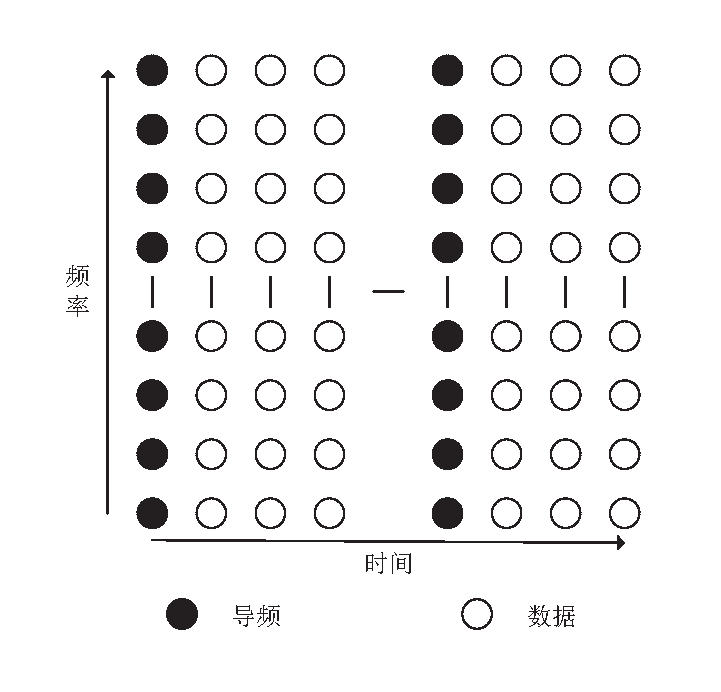
\includegraphics[width = 0.5\textwidth]{figures/Chapter-3/BlockTypePilot.eps}
    }
    \subfloat[梳状导频放置方式]{
        \label{fig:CombTypePilot}
        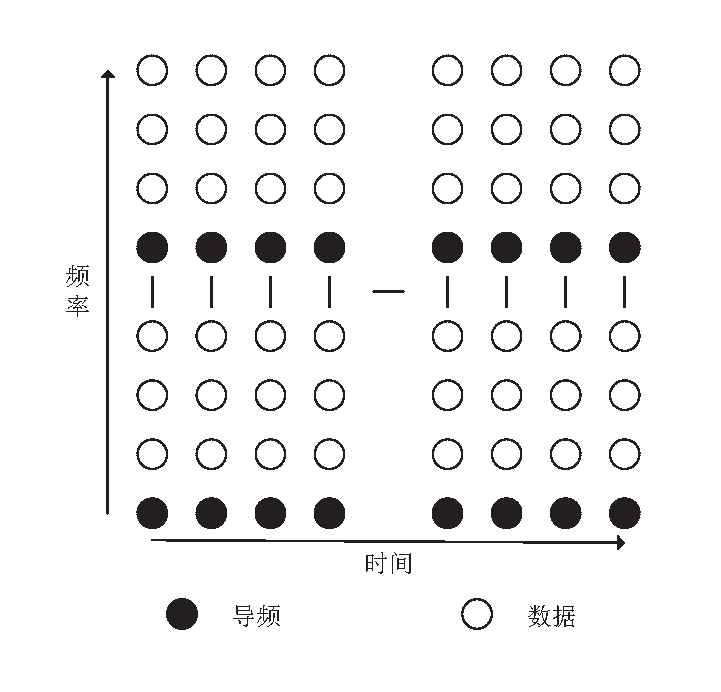
\includegraphics[width = 0.5\textwidth]{figures/Chapter-3/CombTypePilot.eps}
    }
    \caption{导频防止方式}
    \label{fig:PilotAllocation}
\end{figure}



块状导频方式在是在所有的子载波上均放置导频符号,此时这一个OFDM符号不能再放置数据,成为训练序列。
块状导频序列方式适合于在时域慢变换的信道中使用,在一帧数据的第一个符号进行所有子载波的信道估计,其估计结果在一帧数据能都能使用。



\section{本章小结}

本章主要介绍了室内可见光通信系统中两个关键技术——同步和信道估计技术。首先简要介绍了OFDM系统中常用的几类同步算法,
主要针对计算复杂度适中且同步性能优异的基于互相关的同步算法进行了研究,探讨了同步序列的选择标准,
介绍了常见的两种同步序列——ZC序列和PN序列的性能。在研究了同步问题之后,
我们对DCO-OFDM系统的信道估计技术进行了研究,对单色光系统,我们可以采用时域导频或频域导频序列进行信道估计,
而对于多色光通信系统,我们需要设计合理的信道估计方式获得较优的信道估计性能。
对于使用频域导频的信道估计算法,我们介绍了LS估计器和LMMSE估计器,
LMMSE估计相对于LS估计性能更优,但其计算复杂度较高。此外,
还介绍了对LS估计算法的两种改进算法——时域平均算法和频域平均算法,这两种算法计算简单,
但对LS估计性能都有大幅的提升,适合在实际系统中采用。最后我们介绍了使用时域导频干扰抵消的信道估计算法,该算法估计误差小,
性能较优但,其计算复杂度较高。总的来说,较优的信道估计性能和较低的计算复杂度是不能兼得的,我们在设计实际系统需要折衷考虑。


\section{可见光信道估计}
\section{可见光信道非线性分析}
\section{可见光各波段之间串扰估计}
\section{本章小结}
